\documentclass[a4paper, 12pt]{article}
\usepackage[utf8]{inputenc}
\usepackage[T1]{fontenc}
\usepackage[hungarian]{babel}
\usepackage{graphicx}
\usepackage{geometry}
\geometry{a4paper,
		     tmargin = 25mm, 
		     lmargin = 20mm,
		     rmargin = 20mm,
		     bmargin = 20mm}
\usepackage{mathtools}
\usepackage{amsmath}

%Define double underlining
\def\doubleunderline#1{\underline{\underline{#1}}}
% To change the abstract name from the overridden `Kivonat` to `Bevezetés`
\addto{\captionshungarian}{\renewcommand{\abstractname}{Bevezetés}}
% Section numbering
\renewcommand\thesection{\arabic{section}}
\renewcommand\thesubsection{\thesection.\alph{subsection}}

% Laplace and D'Alambert operators
\newcommand*\Laplace{\mathop{}\!\mathbin\bigtriangleup}
\newcommand*\DAlambert{\mathop{}\!\mathbin\Box}

%Vector
\makeatletter
\newcommand{\Spvek}[2][r]{%
  \gdef\@VORNE{1}
  \left(\hskip-\arraycolsep%
    \begin{array}{#1}\vekSp@lten{#2}\end{array}%
  \hskip-\arraycolsep\right)}

\def\vekSp@lten#1{\xvekSp@lten#1;vekL@stLine;}
\def\vekL@stLine{vekL@stLine}
\def\xvekSp@lten#1;{\def\temp{#1}%
  \ifx\temp\vekL@stLine
  \else
    \ifnum\@VORNE=1\gdef\@VORNE{0}
    \else\@arraycr\fi%
    #1%
    \expandafter\xvekSp@lten
  \fi}
\makeatother

\begin{document}

\begin{titlepage}
% Template for future notes.

	\centering
	
\includegraphics[width=0.66\textwidth]{elte.jpg}\par\vspace{1cm}
	{\scshape\LARGE ELTE TTK \par}
	\vspace{2cm}
	{\scshape\Large Az általános relativitáselmélet alapjai\par}
	\vspace{1.5cm}
	{\large\itshape készült az előadások alapján, írta: \par}
	\vspace{1cm}
	{\large\itshape Olar Alex\par}
	\vfill
	oktató\par
	\vspace{0.5cm}
	{\Large Dávid Gyula, \itshape{dgy}}

	\vfill

% Bottom of the page
	{\large 2016/2017 \par}
\end{titlepage}
%%%%%%%%%%%%%%%%%%%%%

\begin{abstract}
Ez a jegyzet \itshape{Dávid Gyula} előadássorozata alapján készült a 2016/17-es tanév második féléveben. A jegyzet bővítése tervben van. Az előadássorozat 3 féléven keresztül végig kíséri a most II. évfolyamot egészen a BSc végéig. Ezen összefoglaló célja számomra az ismétlés, majd közkinccsé tétel. 
\end{abstract}

\vfill

\tableofcontents

\newpage
%%%%%%%%%%%%%%%%%%%%%

\section{Jelölések}
\vspace{1cm}
\hspace{0.5cm} A speciális relativitáselmélet kurzusról ismert jelölésekhez hasonlóan felső és alsó indexeket használunk majd. Ha az index az angol ABC betűje, akkor az 0-3 közötti számozást jelent, ha a görög ABC betűje, akkor csak 1-3 között indexel.
\newline
\begin{center}
$x^{k} = \Spvek{ct;x;y;z} \quad x_{k} = \Spvek{ct;-x;-y;-z} \quad x^{\alpha} = \Spvek{x;y;z} \quad x_{\alpha} = \Spvek{x;y;z}$
\end{center}
\hspace{0.5cm} A tenzorok indexelése hasonlóan felső, alsó, vegyes indexekkel történik.
\begin{center}
$\Lambda^{i j} \quad \Lambda_{i j} \quad \Lambda^{i}_{j}$
\end{center}

\newpage
%%%%%%%%%%%%%%%%%%%%%

\section{Speciális relativitás elmélet - áttekintés}
\vspace{0.5cm} Minden objektum szimmetria csoportjába tartozó transzformációk a:
\begin{itemize}
\item eltolás $\rightarrow$ impulzus megmaradás
\item Lorentz-boost
\item időbeli eltolás $\rightarrow$ energia megmaradás
\item forgatás $\rightarrow$ impulzusmomentum megmaradás
\end{itemize}

\vspace{0.5cm} Az $x^{k}$ koordináták transzformációja ezen szimmetriák alkalmazása.
\begin{equation*}
x'^{k} = \Lambda^{k}_{l}x^{l} + a^{k}
\end{equation*}
\vspace{0.5cm} Ahol $a^{k}$ egy konstans eltolás, míg a két indexes tenzor a Lorentz-transzformációt írja le, a következő alakban:
\begin{equation*}
\Lambda = \left(\begin{array}{cccc} \pm 1&0&0&0 \\ 0& && \\ 0 &&\it{\Large{I}} &\\ 0 && & \end{array}\right)
\left(\begin{array}{cccc} 1&0&0&0 \\ 0& & & \\ 0 & & \it{\large{F}} &\\ 0 &&&  \end{array}\right)
\left(\begin{array}{cccc} \cosh{\chi}&&-\underline{\tilde{n}}\sinh{\chi}& \\ &  && \\ -\underline{n}\sinh{\chi}&&\it{\large{I + (\cosh{\chi} - 1)\underline{n}\circ \underline{n}}}&\\ && & \end{array}\right)
\end{equation*}
\newline
Ahol $I$, $F$ rendre a 3 dimenziós egység és forgás mátrixok.  \newline
\hspace{1cm}
\vspace{0.5cm} A speciális relativitáselméletben a metrikus tenzor rendezi át az indexeket. Ezzel értelmezett a skaláris szorzás is a négyesvektorok között.
\begin{equation*}
x_{k} = g_{kl}x^{l} \quad x^{k} = g^{kl}x_{l} \quad g^{kl}g_{lm} = \delta^{k}_{m}
\end{equation*}
\vspace{0.5cm} A speciális relativitáselméletben a metrikus tenzor saját magának az inverze, konstans.
\begin{equation*}
g_{kl} = \left(\begin{array}{cccc} 1&0&0&0\\ 0&-1&0&0\\ 0&0&-1&0\\0&0&0&-1 \end{array}\right)
\end{equation*}
\vspace{0.5cm} Az ezzel definiált skalárszorzás pedig.
\begin{equation*}
x^{k}x_{k} = g_{kl}x^{k}x^{l} = (ct)^{2} - x^{2} - y^{2} - z^{2}
\end{equation*}
Az általános relativitáselmélet célja, hogy lokálisan teljesítse a speciális relativitáselméletet, viszont globálisan egy új leírást adjon a világra.
\newpage
%%%%%%%%%%%%%%%%%%%%%%%%%

\section{Newtoni - gravitáció}
A newtoni gravitáció elmélete az évszázadok során beleivódott minden ember tudatába. A távolba hatás, a távoli testek által egymásra kifejtett erő mind-mind alapfogalmak a fizika tanulás kezdetén. \newline
A mozgásegyenletekben szereplő arányossági tényezők egyenlősége komoly mérési eljárások kidolgozásra révén volt bizonyítható, súlyos tömeg, tehetetlen tömeg.
\begin{equation*}
m_{t}\vec{a} = m_{s}\vec{g}(\vec{r},t)
\end{equation*}
Kísérleti tény az is, hogy zárt görbén a gravitációs erőnek nincsen munkája. Azaz:
\begin{equation*}
\oint_\gamma \vec{g}(\vec{r},t) \,d\vec{r} = 0 = \int_F (\nabla \times \vec{g}) d\vec{F} = 0 \quad \quad \rightarrow \quad \quad \nabla \times \vec{g} = \vec{0}
\end{equation*}
Ebből következik, hogy $\vec{g}$ egy skalármező negatív gradienseként előállítható. Így:
\begin{equation*}
\oint_{\partial V} \vec{g} d\vec{F} = \int  \nabla\vec{g}dV = - 4\pi G \int \rho(\vec{r})dV \quad \rightarrow \quad \nabla\vec{g} = -4\pi G\rho(\vec{r})
\end{equation*}
Így látható, hogy folytonos tömegeloszlásra a Newton-féle gravitációs törvény a következő alakot ölti.
\begin{equation*}
\vec{g} = -\nabla\Phi \quad \rightarrow \quad \Laplace\Phi = 4\pi G \rho(\vec{r})
\end{equation*}
Az utóbbi lényegében a gravitációra felírt Poisson-egyenlet. \newline
\hspace{0.5cm} Áttérve a speciális relativitáselméletre a gravitációs erő általánosítása a következő egyenlet lenne:
\begin{equation*}
\frac{d}{d\tau}(Mu_{k}) = M \partial_{k}\Phi
\end{equation*}
A sajátidő ($\tau$) szerinti deriválást elvégezve és kihasználva, hogy a négyessebesség $u_{k}u^{k} = c^{2}$ a következő összefüggést kapjuk:
\begin{equation*}
\frac{dM}{d\tau}c^{2} = \frac{\partial \Phi}{\partial x^{k}} \frac{dx^{k}}{d\tau}M = \frac{d\Phi}{d\tau}M
\end{equation*}
Ezt nevezhetjük a \textsc{Novobátzky-effektus}  speciális esetének. Mivel ez egy szeparálható differenciál egyenlet, a megoldása előáll
\begin{align*}
M = m e^{\frac{\Phi(x^{k})}{c^{2}}}
\end{align*}
Ezt pedig $1911$-ben \textsc{Nordström} vezette le. Lényegében ez volt a legjobb gravitáció elmélet amit a speciális relativitás elmélet előállított. A korábbiak alapján a mozgásegyenlet is előállítható, ha a kezdeti egyenletbe visszahelyettesítjük a $\frac{dM}{d\tau}$ tagot.
\begin{equation*}
\frac{dM}{d\tau} = \frac{1}{c^{2}}Mu^{l}\partial_{l}\Phi \quad \rightarrow \quad (\delta^{l}_{k} - \frac{u^{k}u_{l}}{c^{2}})\partial_{l}\Phi = \frac{du_{k}}{d\tau}
\end{equation*}
Jól látható, hogy a potenciál gradiense előtt álló operátor egy, a négyessebességre merőleges vetítést hajt végre.
\section{Alapfogalmak}
\hspace{0.5cm} Az első féléves mechanika és az Elméleti mechanika tárgyak szerves részét képezi a gyorsuló koordináta-rendszerek vizsgálata. Mind ismerjük a kulcsfogalmakat. Szükség van egy rögzített koordináta-rendszerre amihez képest egy másik origója $a_{0}$ gyorsulással transzlációt végezhet és foroghat. A forgás leírására a koordináta-rendszerek közötti ortogonális transzformációt használjuk, ahol az ortogonális mátrixok időfüggőek.
\begin{equation*}
\doubleunderline{\dot{O}}\hspace{0.1cm}\doubleunderline{O}^{T} = \doubleunderline{\Omega} = \underline{\omega} \times
\end{equation*}
A mozgásegyenlet pedig a következőképen transzformálódik:
\begin{equation*}
m\underline{a} = \underline{F} + m\underline{a}_{0} + m \underline{\omega} \times (\underline{\omega} \times \underline{r}) + 2m\underline{\omega}\times\underline{\dot{r}} + m \underline{\dot{\omega}}\times \underline{r}
\end{equation*}
\textsc{Einstein} arra jött rá, hogy a gravitáció sem erő, hanem egy koordináta transzformációval eltüntethető jelenség. Ennek leírására segítséget kért egy Magyarországon született, matematikus barátjától, \textsc{Marcell Grossmann}tól. Együtt dolgozták ki az általános relativitáselmélet matematikáját a \textsc{Riemann-féle differenciálgeometria} alapján. \newline
\par A kulcsgondolatok:
\begin{itemize}
\item Nincs globális koordináta-rendszer amihez viszonyítani lehetne a lokális rendszereinket.
\item Lokális rendszereink Minkowski-geometriájúak, azaz lokálisan a speciális relativitáselmélet teljesül.
\end{itemize}
\par
Ennek precíz matematikai leírásához a következő gondolati lépesek lennének szükségesek:
\begin{enumerate}
\item halmaz $\rightarrow$ ezen értelmezett folytonosság, differenciálhatóság
\item konnexió (kapcsolat a topologikus tér és a metrikus tér között)
\item metrika
\end{enumerate}
A leíráshoz a sokaságok elméletét fogjuk alapul venni. Ezek közül is nekünk a differenciálható részsokaságok egy speciális részhalmaza kell majd a tér-idő leíráshoz. Hiszen mit tud egy fizikus? \textsc{Deriválni.}
\subsection{Affin tér:}
Egy affin tér egy (V, \textbf{V}, \textbf{-}) hármas, ahol:
\begin{itemize}
\item V nem üres halmaz
\item \textbf{V} vektortér
\item ''\textbf{-}'' leképezés pedig V  $\times$ V $\rightarrow$ \textbf{V}, amit (x,y) $\mapsto$ x-y = $\vec{a}$ alakban írunk
\end{itemize}
Axiómái a következők:
\begin{itemize}
\item (x-y) + (y-z) + (z-x) = $\vec{0}$
\item az affin tér és az alul fekvő vektortér dimenziója azonos
\item $\vec{a}$ = A \textbf{-} $o$ leképezést az affin tér $o$ középpontú ortogonalizációjának nevezzük
\end{itemize}
A tér-időről kezdetben csak annyit feltételezünk, hogy az egy 4 dimenziós affin tér, amely lokálisan Minkowski-struktúrával van ellátva. Ezeket a különböző rendszereket kell majd valahogy összefésülni.
\subsection{Metrika}
\par Legyenek $a$,$b$ egy $\textsl{M}$ halmaz elemei. Ekkor a $\rho : \textsl{M} \times \textsl{M} \rightarrow \textsl{R}$ hozzárendelést metrikának nevezzük, ha:
\begin{itemize}
\item $\rho(a,b) \geq 0$, valamint akkor és csak akkor $0$, ha $a = b$
\item $\rho(a,b) = \rho(b,a)$
\item $\rho(a,b) \leq \rho(b,c) + \rho(c,a)$
\end{itemize}
\par A sokaságok leírásához viszont egyenlőre nem metrikát használunk. Mások lesznek az alapfogalmaink. A $\textsc{nyílt halmaz}$ok lesznek az alapfogalmaink. Erre építünk majd mindent, még ha nem is a lehető legprecízebb módon. Az $\textsl{Analízis I.}$ kurzusról már ismeretesek a nyílt halamzokra vonatkozó alapállítások:
\begin{itemize}
\item Végtelen sok nyílt halmaz uniója nyílt.
\item Véges sok nyílt halmaz metszete is nyílt.
\end{itemize}
\par Legyen $X$ egy halmaz, ennek nyílt részhalmazai $B$-k. Az ezeket tartalmzó struktúrát ekkor $\textsc{topologikus tér}$nek nevezzük, ha tartalmazza $X$-et, az üres halmazt, valamint a nyílt halmazok végtelen unióját és véges metszetét. A topologikus tér ezáltal egy olyan halmaz, amin a folytonosság értelmezve van, hiszen tudunk közelséget/szomszédságot definiálni. Gyakorlatban persze a fizikus nem absztrahál ennyire, visszanyúl a koordinátázáshoz.
\par Vegyükn egy sokaságot, legyen ez $\textsl{M}$. Ennek két részhalmazát $U$,$V$, melyek metszete nem üres képezzük le egy  rendre $p$,$q$: $\textsl{M}$  $\rightarrow$ $\textsl{$R^{n}$}$ paraméterezésekkel. Ekkor a közös metszes leképződött $\textsl{$R^{n}$}$ két részhalmazára amik között értelmezhető egy $F$ : $\textsl{$R^{n}$}$ $\rightarrow$ $\textsl{$R^{n}$}$ leképezés, amit kiterjeszthetünk $U$-ról, $V$-re, feltéve, hogy a paraméterezések invertálhatóak. Tehát $F$$\circ$ $q^{-1}$ $\circ$ $p$ : $U$$\rightarrow$ $V$ függvény már a sokaságon értelmezett. Megmutatható, hogy ez a paraméterezéstől független. 
\par Az ilyen leképzesésekkel értelmezhető az absztrakt sokaságon a foyltonosság és deriválhatóság, hiszen $F$-en már ezeket könyedén tudjuk értelmezni. A keletkezett téképlapok maguk fölé definiálnak egy sokaságot. Ezt nevezzük $\textsc{algebrai topológiának}$, értelmezhetővé válik a differenciálható sokaság fogalom. Tartsuk szemelőtt, hogy $\textsl{továbbra sincsen beágyazó tér}$ (matematikusok belátták, hogy nem triviális módon értelmezhető olyan tér, amibe beágyazható egy ilyen struktúra, de ez közelében sincs a hétköznapi fogalmainknak). 
\newline
\begin{center}
\par $\textit{Eljutottunk tehát oda, hogy ki tudjuk mondani, hogy a $\textsc{téridő modell}$ünk egy olyan}$ \newline $\textit{$4$ dimenziós differenciálható sokaság, amely lokálisan Minkowski-tér.}$
\end{center}
\par Az általános relativitáselméletben csakis felső indexes ''vektrok'' lesznek, mivel ezek a görbevonalú koordinátázáshoz képest, nem vektrokomponensek, hanem pusztán $\textsc{koordináták}$. Tehát nem transzformálódnak homogén lineáris módon.
\par Már értelmezhetünk skalármezőt is. Általánosságban csak mezőket tudunk majd értelmezni amúgy is, hiszen az elmélet csak minden a sokaság minden pontjában értelmezett objektumokat enged meg. Legyen tehát $\Phi : \textsl{M} \rightarrow \textsl{R}$, mivel $\textsl{P}$ pont kölcsönös egyértelmű viszonyba hoszható a térképzeésen egy $x^{k}$ koordinátával így a (fizikus módon ugyan azzal a betűvel jelölve) $\Phi : \textsl{$R^{n}$} \rightarrow \textsl{$R^{n}$}$ függvény már egy skalármezőt definiál $\textsl{M}$-n is.
\newline
\par $\textsl{Einstein}$ célja a gyorsuló koordinátákra való kovariáns áttérés matematikai leírása és fizikai megalapozása volt.
\par Ha ugyan arról a részsokaságról készítünk különböző térképzeéseket, akkor azok között léteznie kell egy folytonos, differenciállható és invertálható leképzésnek, ami ezeket egymásba transzformálja.
\section{Topológia, derivációk, metrika}
\par Legyen a sokaság minden pontjában értelmezve egy $T_{p}$ vektortér ( - érintőtér - ), ami független a paraméterezéstől mégis annak segítségével definiálhatjuk, hiszen ezeket a paraméterezés deriváltjának az értékkészletének egy részén értelmezhetjük:
\begin{equation}
T_{P}(\textsl{M}) := Ran_{Dp(p^{-1}(x))}
\end{equation}
Az ezen pontokban vett érintőterek unióját $\textsc{tangens nyaláb}$nak nevezzük. Ennek $\textsl{szelése}$ egy vektormező, ami lényegében egy olyan művelet, ami minden ponthoz hozzárendel az adott pontban vett érintőtérből egy elemet. Mivel a vektromező minden egyes eleme más halamzból került ki, így a különböző lineáris terek közötti átszámítás nem triviális. Egy szemléltetést segítő ábra erről:
\begin{figure}[h!]
\centering
\begin{minipage}{0.46\linewidth}
\centering
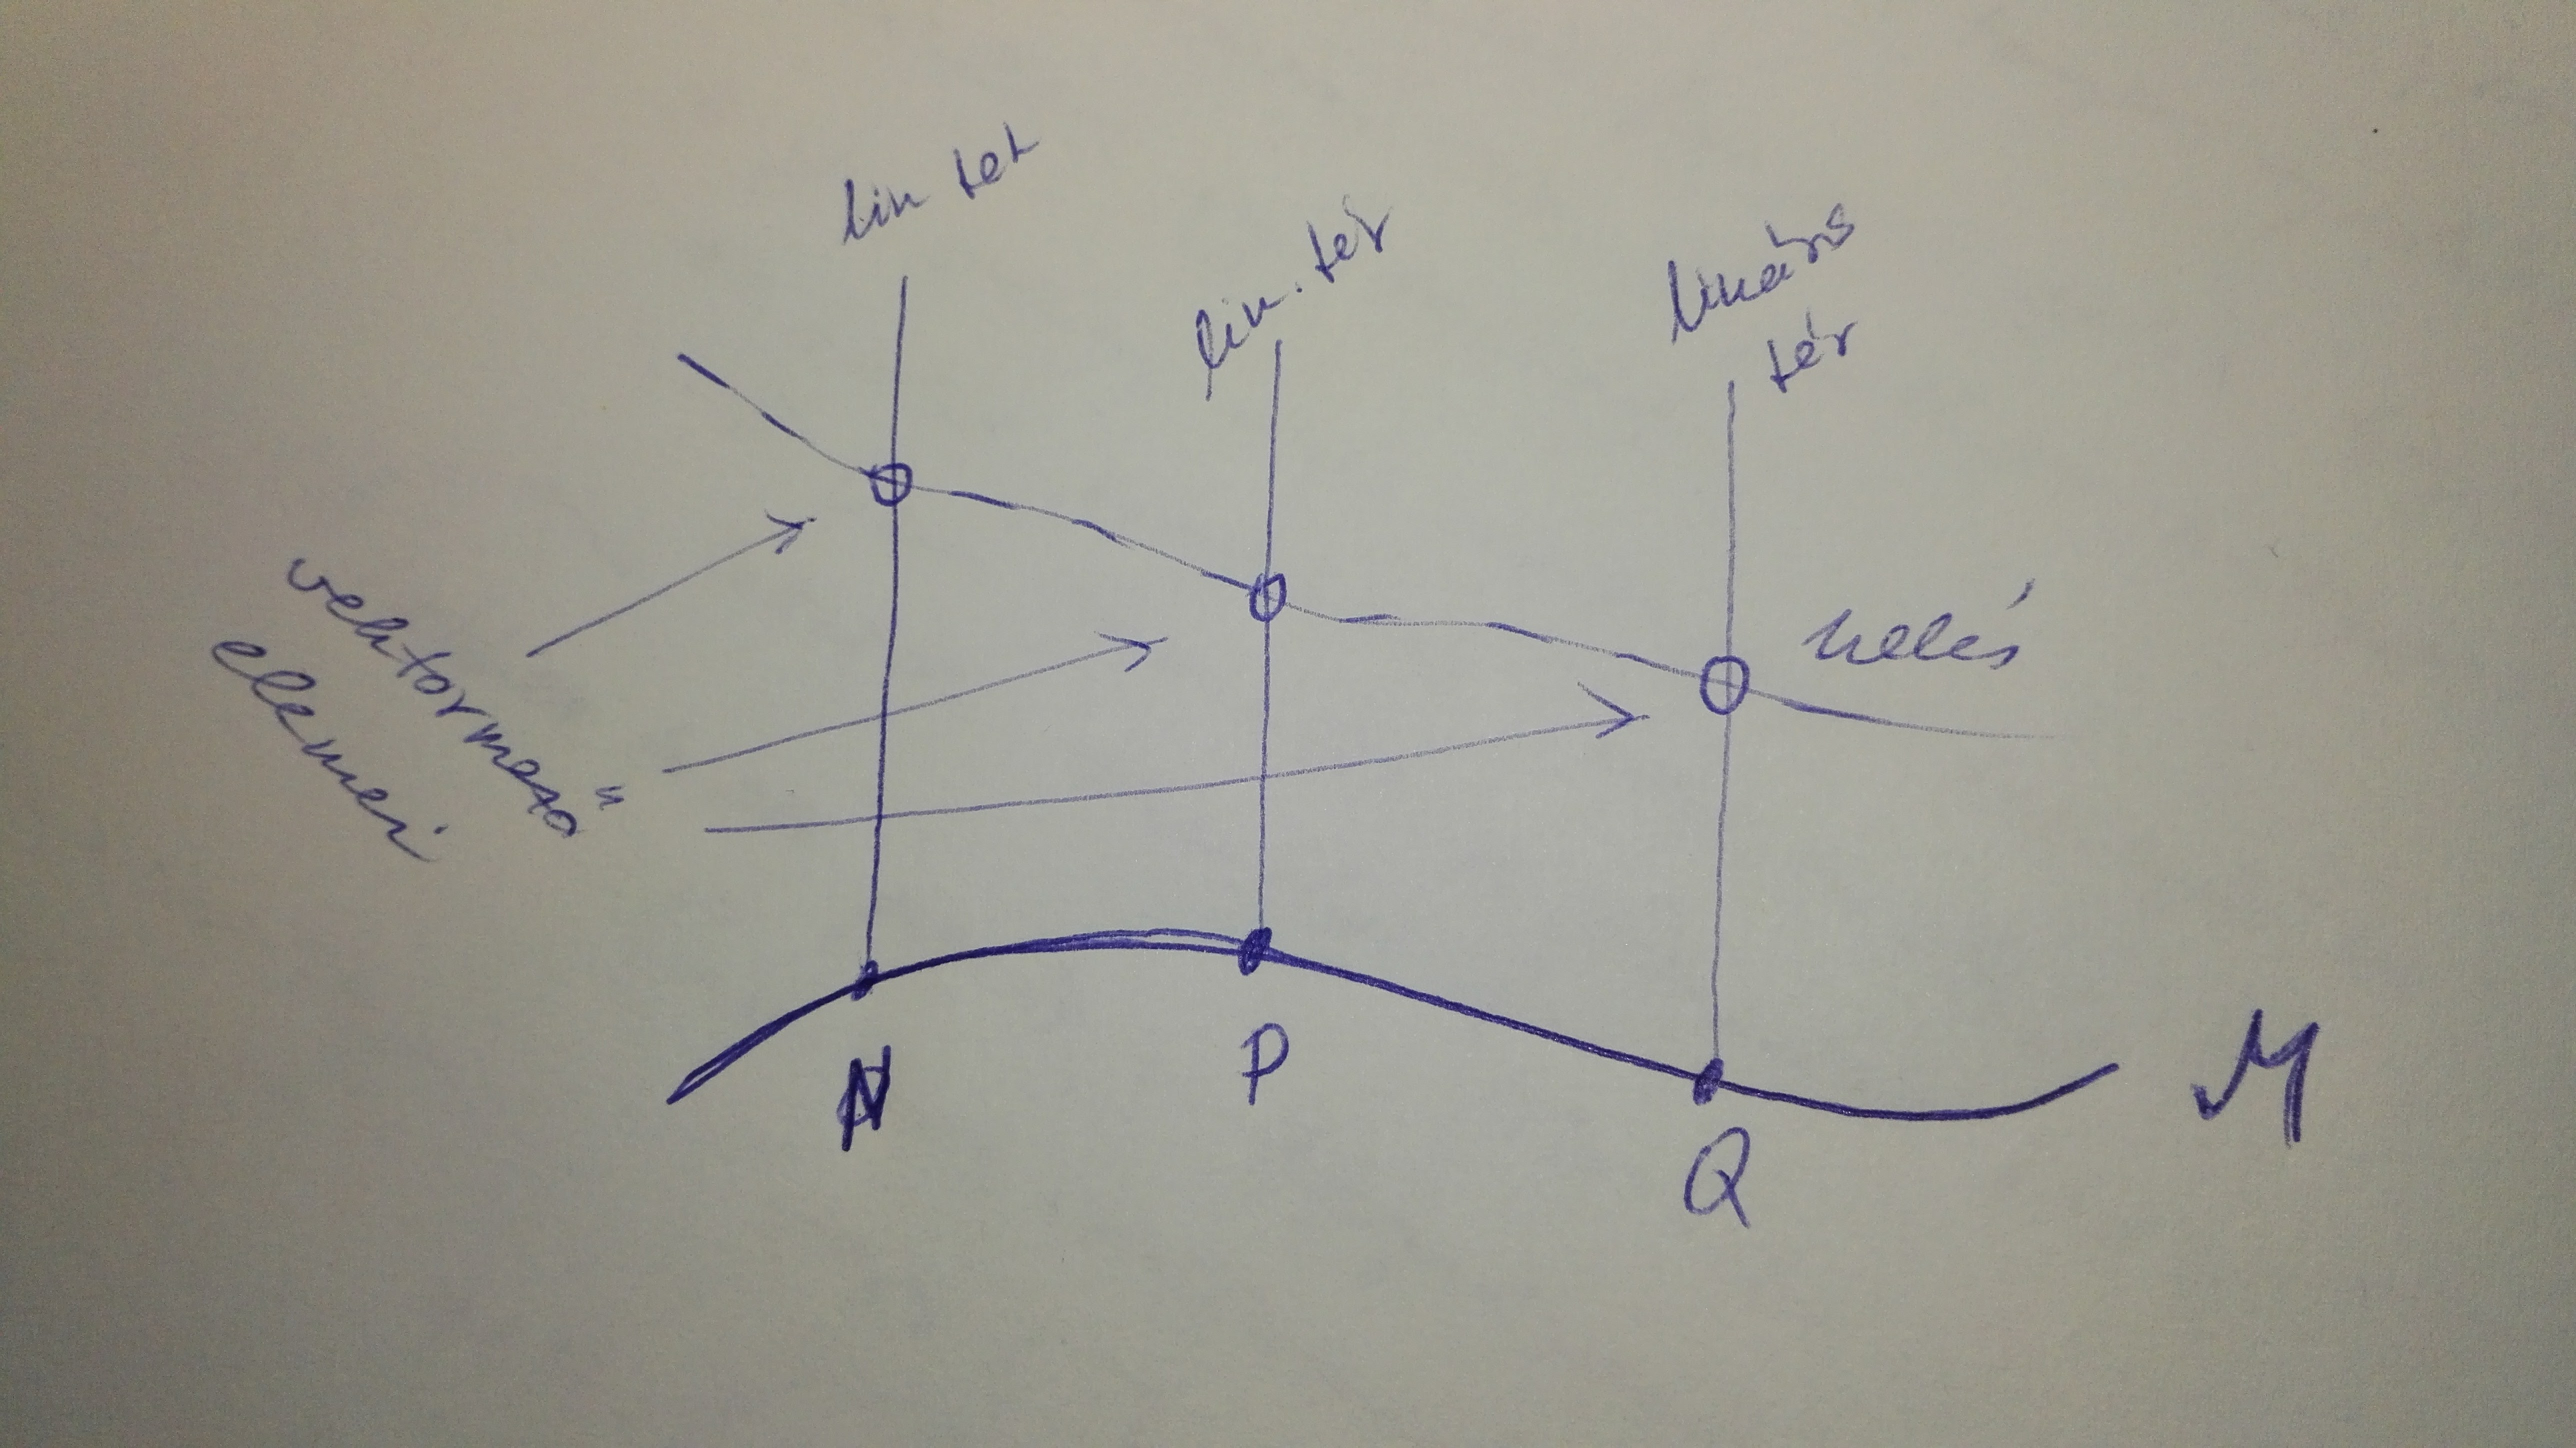
\includegraphics[width=0.9\linewidth]{szeles.jpg}
\caption{Szelés szemléltetése}
\end{minipage}
\begin{minipage}{0.46\linewidth}
\centering
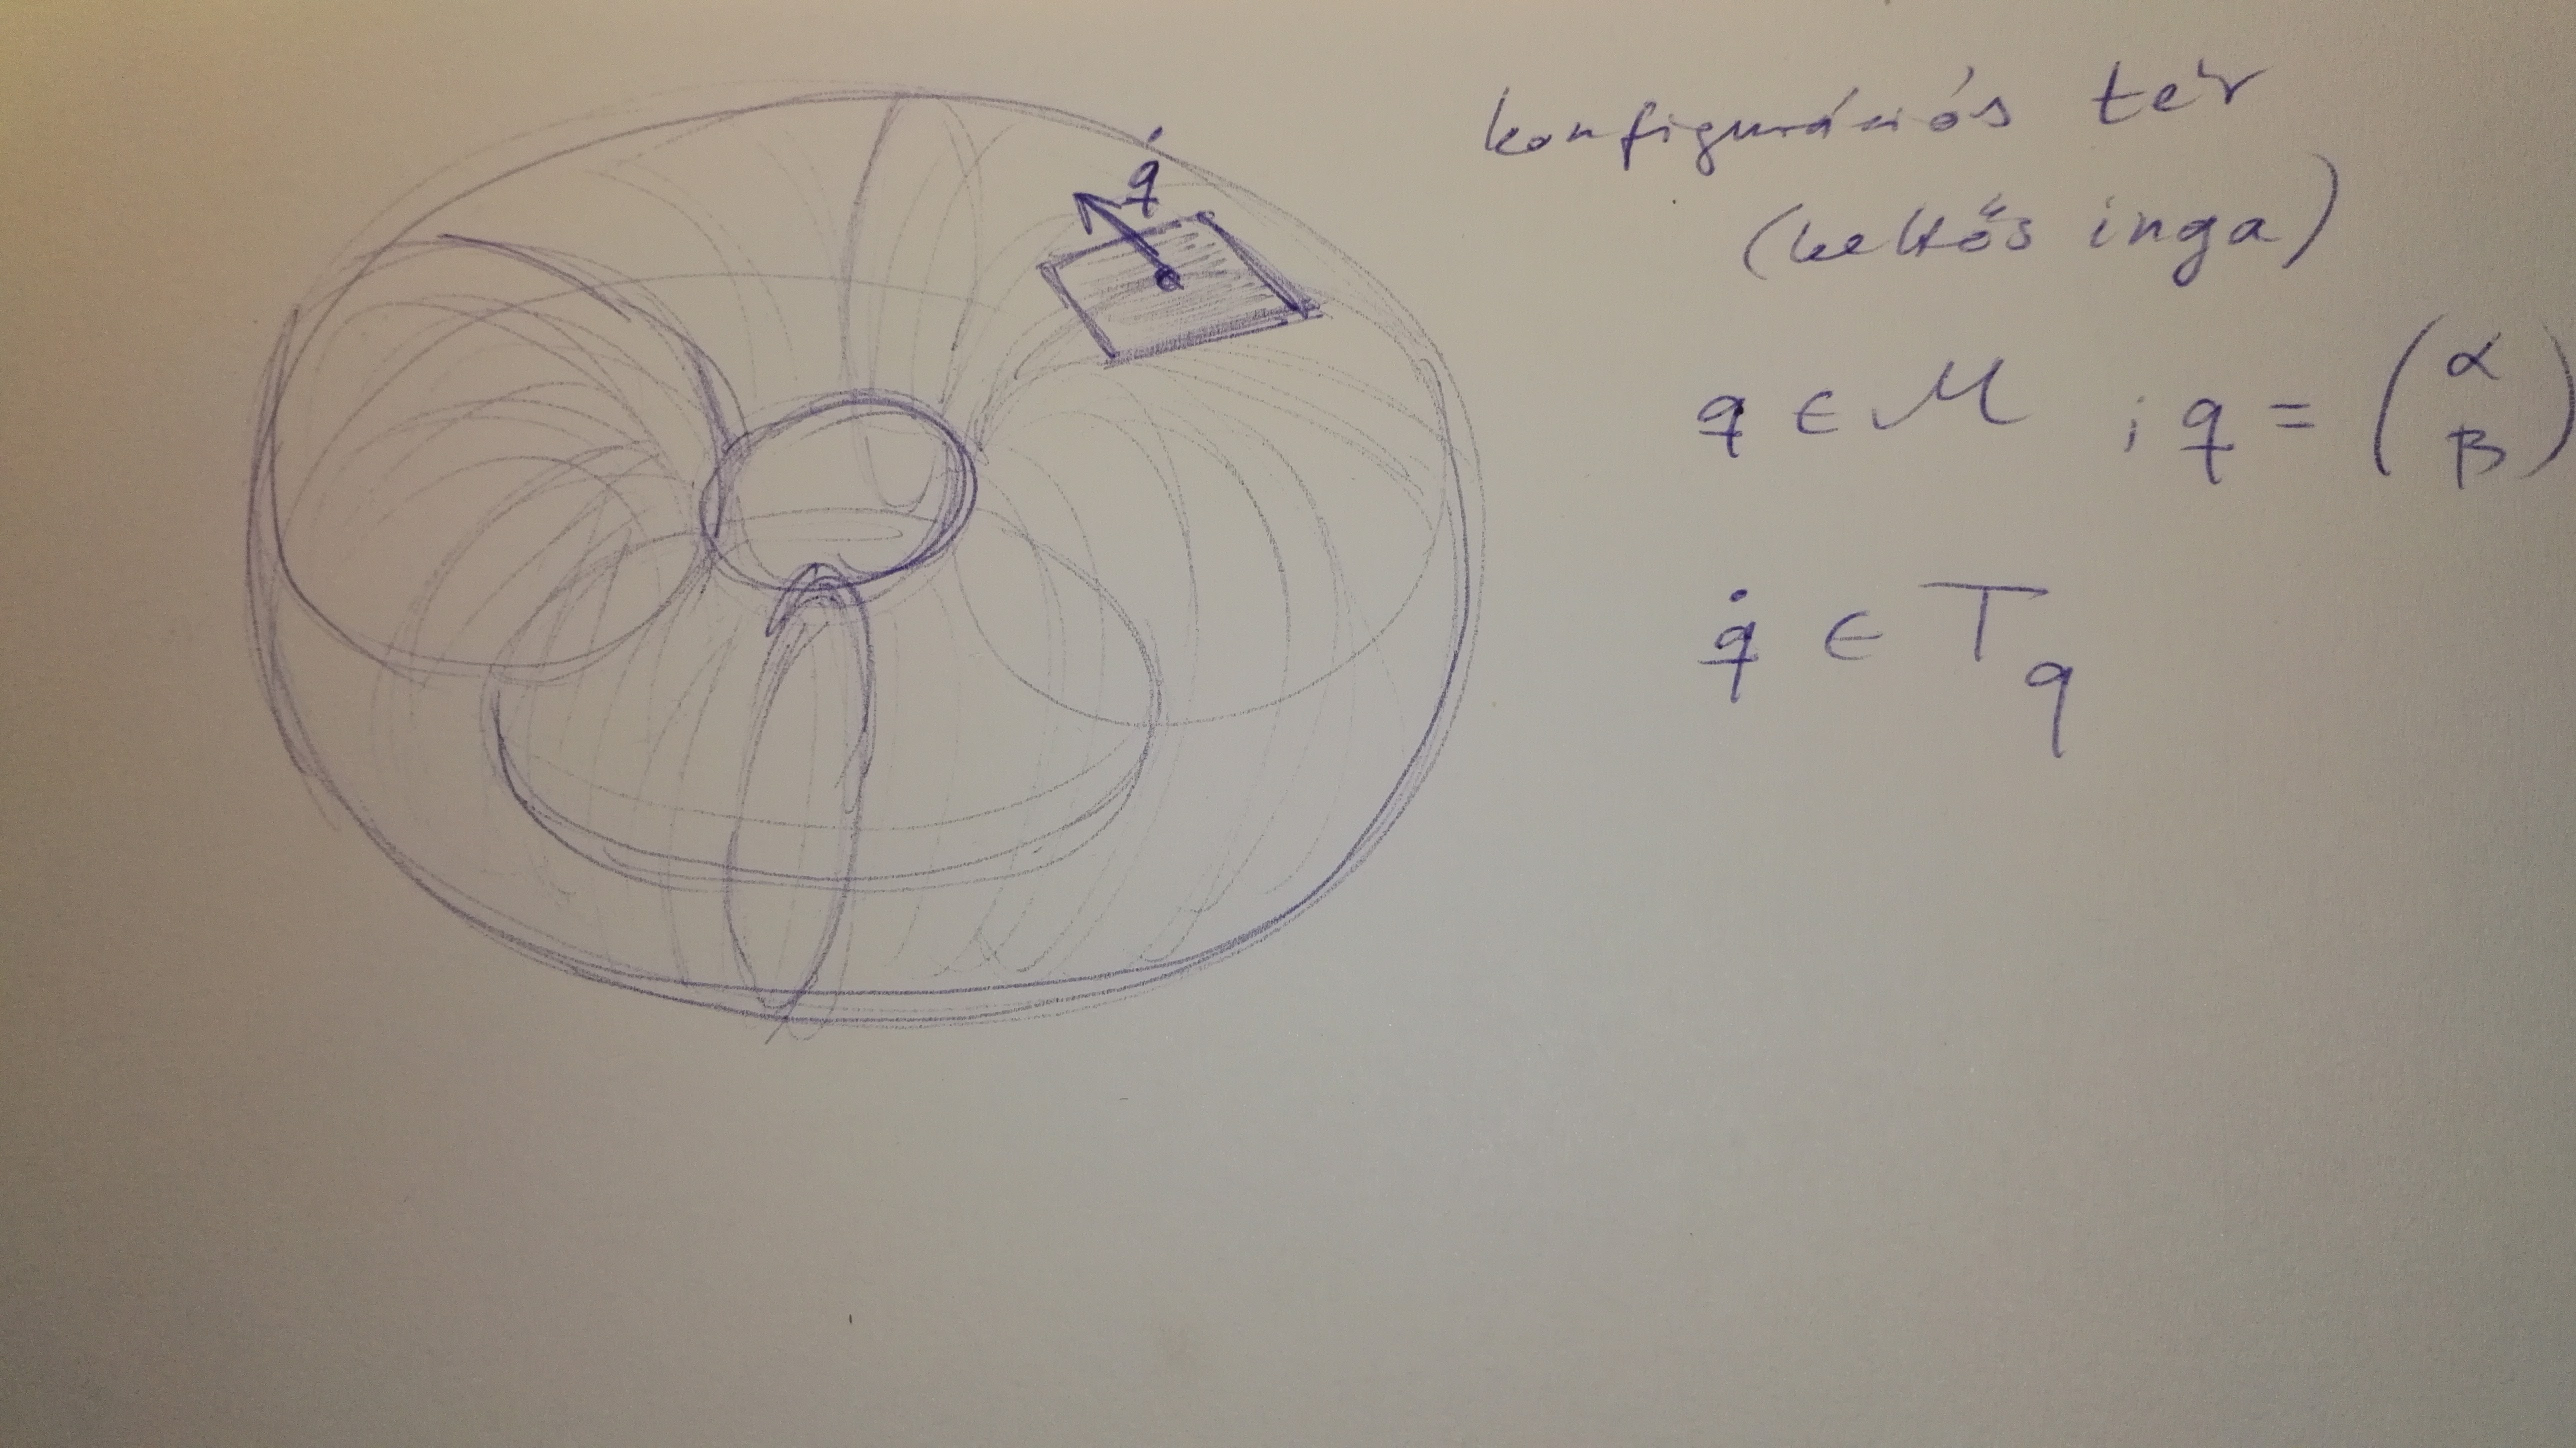
\includegraphics[width=0.9\linewidth]{konfi.jpg}
\caption{Konfigurációs tér}
\end{minipage}
\end{figure}
\par Ahol az utóbbi a kettős inga konfigurációs terén értelmezett érintőtér, vagyis az általános koordináták deriváltja. Tehát lényegében a Lagrange-függvény a konfigurációs tér érintőterén értelmezett függvény.
\newline
\par A sokaság lokálisan $\textsl{homeomorf}$ $R^{n}$-el. Azaz kölcsönösen egyértelműen és folytonos leképezhető, persze csak akkor ha $n$ véges. A sokaság olyan topologikus tér, amely mindenhol lokálisan homeomorf $R^{n}$-el. Topologikus struktúránk tehát már van, de távolság fogalom még mindig nincs a sokaságon értelmezve.
\subsection{Duális terek fogalma}
\par Legyenek ($V_S$,+,*), valamint ($W_S$,+,*) vektorterek ugyanazon skalártest felett és $\textsl{A} : V \rightarrow W$ lineáris leképezés. Ezeken értelmezett az összeadás és a számmal szorzás így lineráis teret alkotnak az operátorok is.  Mi most egy speciális esetet vizsgálunk, amikor is $W_S = S$, mivel ekkor a lineáris leképezéseink funkcionálok, vagyis egy vektortérből skalárhalmazba képező függvények (lineritás továbbra is fennáll természetesen).
\par A továbbiakban $S$ megegyezik a valós számok halmazával. Mostantól pedig a teret, amelyben a funkcionáljaink laknak hívjuk a $V$-hez tartozó $V^{*}$ duális térnek, vagy röviden $V$ duálisának. A funkcionálok lineáris teret alkotnak:
\begin{itemize}
\item $\varphi, \psi \in V^{*}$, valamint $x \in V$ és $\alpha \in R$
\item $(\varphi + \psi)x = \varphi x + \psi x$
\item $(\alpha \varphi)x = \alpha (\varphi x)$
\end{itemize}
\par Ahhoz, hogy erről a duális térről megállapítsuk, hogy hány dimenziós válasszunk benne egy bázist. Legyenek $\{\vec{e}_{k}\}_{k = 1}^{n}$ $\in$ $V$. Bármelyik $\vec{a} \in V$ előáll ezek lineárkombinációjaként. Ekkor:
\begin{align*}
\varphi\vec{a} = \varphi(a^{k}\vec{e}_{k}) = a^{k}\varphi\vec{e}_{k} \quad  \quad a^{k} \in R \\
\varphi\vec{e}_{k} = \varphi_{k} \in R
\end{align*}
tehát a funcionált is n darab adattal tudjuk reprezentálni. Bevezetve speciális $\epsilon^{k} \in V^{*}$ olyan, hogy $\epsilon^{k}\vec{e}_{l} = \delta_{l}^{k}$. Ha előállítunk egy $\Phi \in V^{*}$ funkcionált a következő módon:
\begin{align*}
\Phi = \varphi_{k}\epsilon^{k} \in V^{*} \\
\Phi\vec{a} = \varphi_{k}\epsilon^{k}\vec{a} = \varphi_{k}a^{k} = \varphi\vec{a} \\
\rightarrow \Phi = \varphi \in V^{*}
\end{align*}
\par Vagyis ez azt jelenti, hogy véges dimenziós esetben a vektortér bázisai kölcsönösen megfeleltethetőek a duális térben $\epsilon^{k}$ bázisoknak így $dimV = dimV^{*}$ feltétel teljesül. Emelett elfogadjuk, hogy egy vektortér duálisának a duálisa a kezdeti vektortér, valamint, hogy egy vektortér és duálisa izomorfak.
\newline
\par Most, hogy már bevezettük a duális terek fogalmát vegyük észre, hogy egy adott vektorhoz a duális térből rendelt elem önkényes, valamilyen előre definiált válaszott művelet kell hozzá. Legyen $\vec{a} \in \textsl{V}$, ahol adott bázis mellett $\vec{a} = a^{k}\vec{e}_{k}$. Rendeljük ehhez a duális tér egy $b$ elemét, ahol szintén bázisválasztás után, $b = b_{k}\epsilon^{k}$. Ez a hozzárendelés önkényes, hiszen most definiáljuk, hogy legyen $b_{k} = g_{kl}a^{l}$ és ezentúl jelölésben pedig $b = a^{+}$ használunk majd. Itt $g_{kl}$ a $\textit{metrikus tenzor}$. Ezzel már értelmezhető az elemek közötti skaláris szorzás.
\subsection{Derivációk}
\par Legyenek $\Phi, \Psi : \textsl{M} \rightarrow \textsl{R}$ skalármezők. Legyen továbbá $\sum$ az ilyen skalármezők halmaza. Ezen értelmezve van a mezők számmal szorzása, a mezők összege, és a mezők egymással való szorzása is.
\par Legyen $D : \sum \rightarrow \sum$ lineáris leképezés és legyen a neve $\textsl{DERIVÁCIÓ}$. A művelet szamábalyi a követekező képpen fogalmazhatóak meg:
\begin{itemize}
\item $D(\alpha\Phi + \beta\Psi) = \alpha(D\Phi) + \beta(D\Psi)$
\item $D(\Phi\Psi) = (D\Phi)\Psi + \Phi(D\Psi)$
\end{itemize}
\par A derivációk vektorteret alkotnak. Lévén, hogy $\alpha D_1 + \beta D_2$ is deriváció.
\newline
\par Hogyan is lehet ezeket elképzelni? Először is, olyan művelet kell, ami skalármezőből, skalármezőt csinál. Lineárisnak kell lennie és vektorteret kell alkosson. Ki kell elégítenie a megadott követelményeket is. Vegyük észre, hogy nem véletlen a név, hiszen a fentebbi szabályok is valami féle deriválásra utalnak. Jó példa lehet a deriváció műveletére a $\underline{v}\hspace{0.1cm}\underline{\nabla}$ operáció. 
\par Vizsgáljuk egy adott pontban az ott átmenő összes görbét., legyenek ezek $\underline{r}_{1}(t_1), \underline{r}_{2}(t_2), ...$. Ezeket úgy paraméterezzük, hogy $t = 0$ időpillanatban legyen az összes $\underline{R}$. Minden pontban értelmezve van $\dot{\underline{r}}_{k}(t)$ és adott pontban lineáris teret alkot ezek összessége. Adott pontban tehát $\dot{\underline{r}}_{k}(t_k)\nabla$ operáció deriváció. A probléma csupán az, hogy ez nagyon szemléletesen definiálható $\textsl{R}^{n}$-ben, de nekünk most ugyan ez kéne a sokaságon. Ismét ahhoz folyamodunk, hogy az absztrakt halmazon úgy defináljuk ezeket, hogy az a térképezéseknek és paraméterezéseknek eleget tegyen. 
%%% Ezt a részt annyira nem értem. Át kéne beszélnem a többiekkel, meg jó lenne ha fenn lennének már a videók...
\par Így bevezethetünk egy:
\begin{equation*}
    \Psi = v_{k}\partial_{k}\Phi = \dot{r}_{k}\partial_{k}\Phi = \frac{dx_{k}}{dt}\partial_k\Phi \quad \quad \rightarrow \frac{dx_{k}}{dt}\partial_{k}
\end{equation*}
\par Ahol $\frac{dx_{k}}{dt}\partial_{k}$ definiál a sokaság minden pontjában egy vektorteret. Ezt nevezzük a sokaság adott pontbeli érintő terének. Lényegében a $\partial_{k}$-k az adott pontbeli vektor tér bázis vektorai. Ez szemléletesen azt jelenti, hogy ha egy változót kiválasztunk, akkor az aszerint vett parciális derivált a sokaságon kijelöl görbéket, amelyeket azon változó változtatása mellett a többit állandóan tartva kaptunk. Adott pontban az össze deriváció előállítható a deriválások lineáris kombinációjaként.
\begin{figure}[h!]
\centering
\begin{minipage}{0.46\linewidth}
\centering
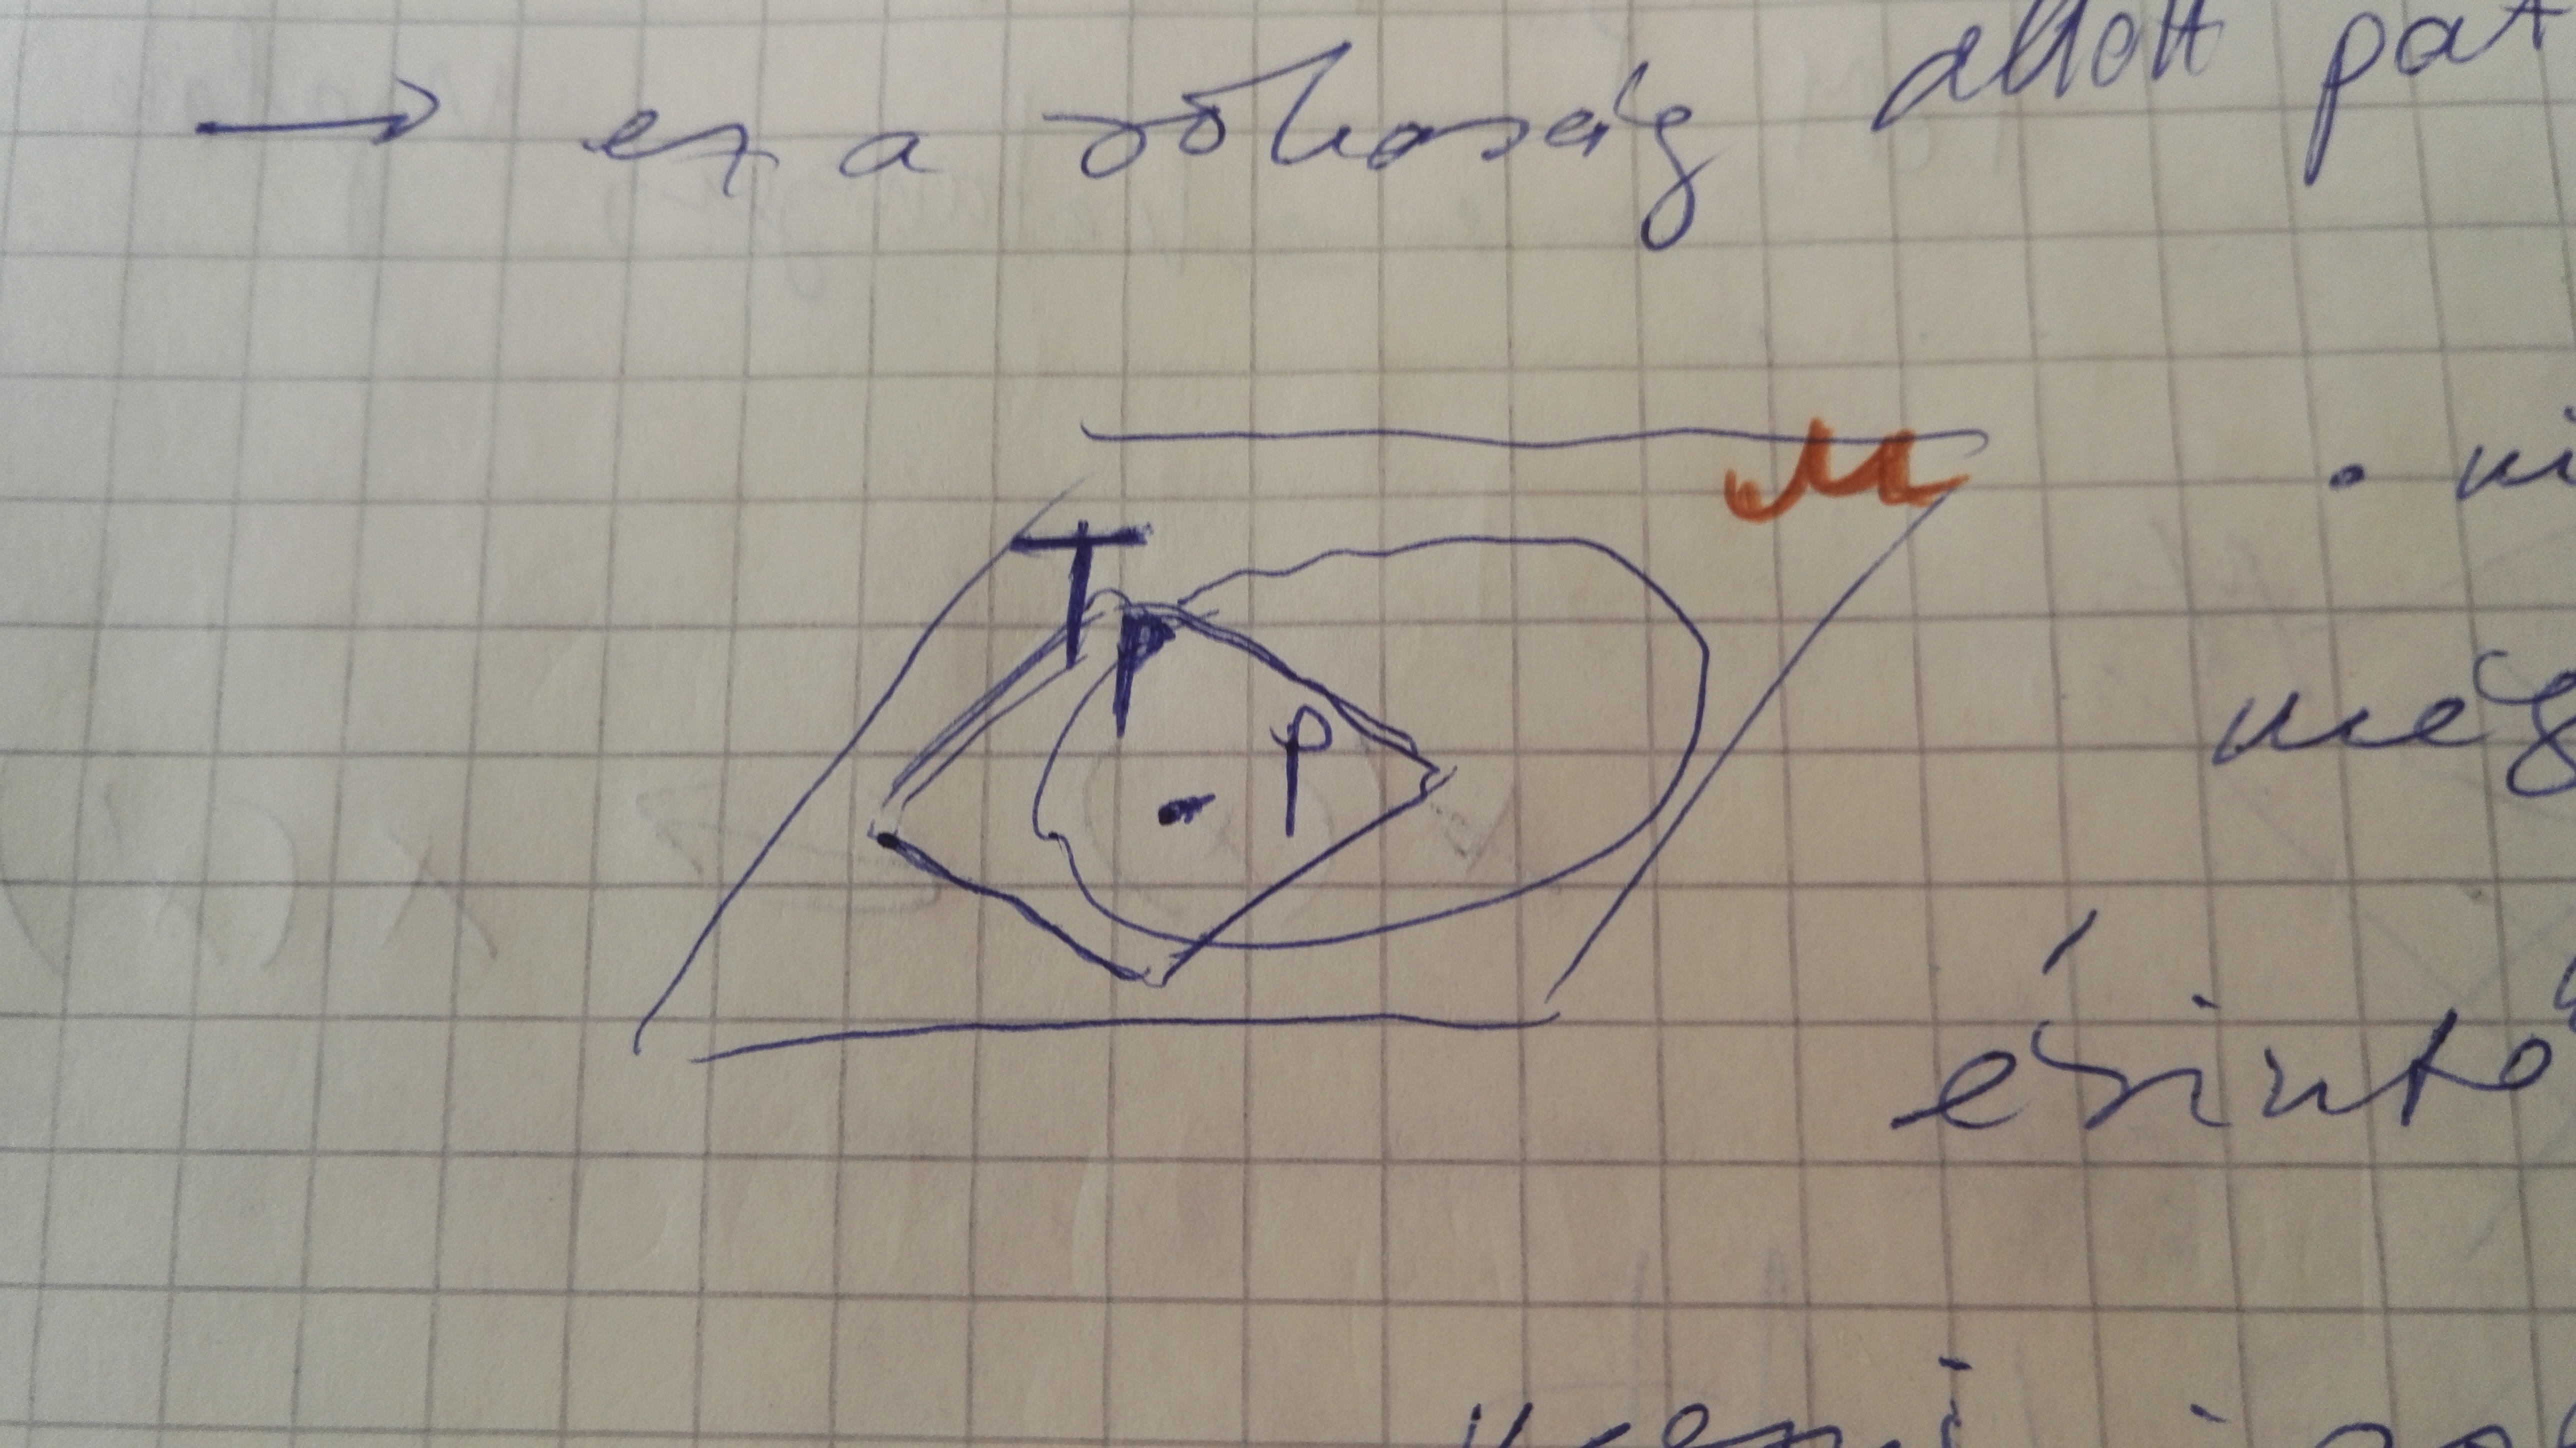
\includegraphics[width=0.9\linewidth]{erintoter.jpg}
\caption{Érintőtér}
\end{minipage}
\begin{minipage}{0.46\linewidth}
\centering
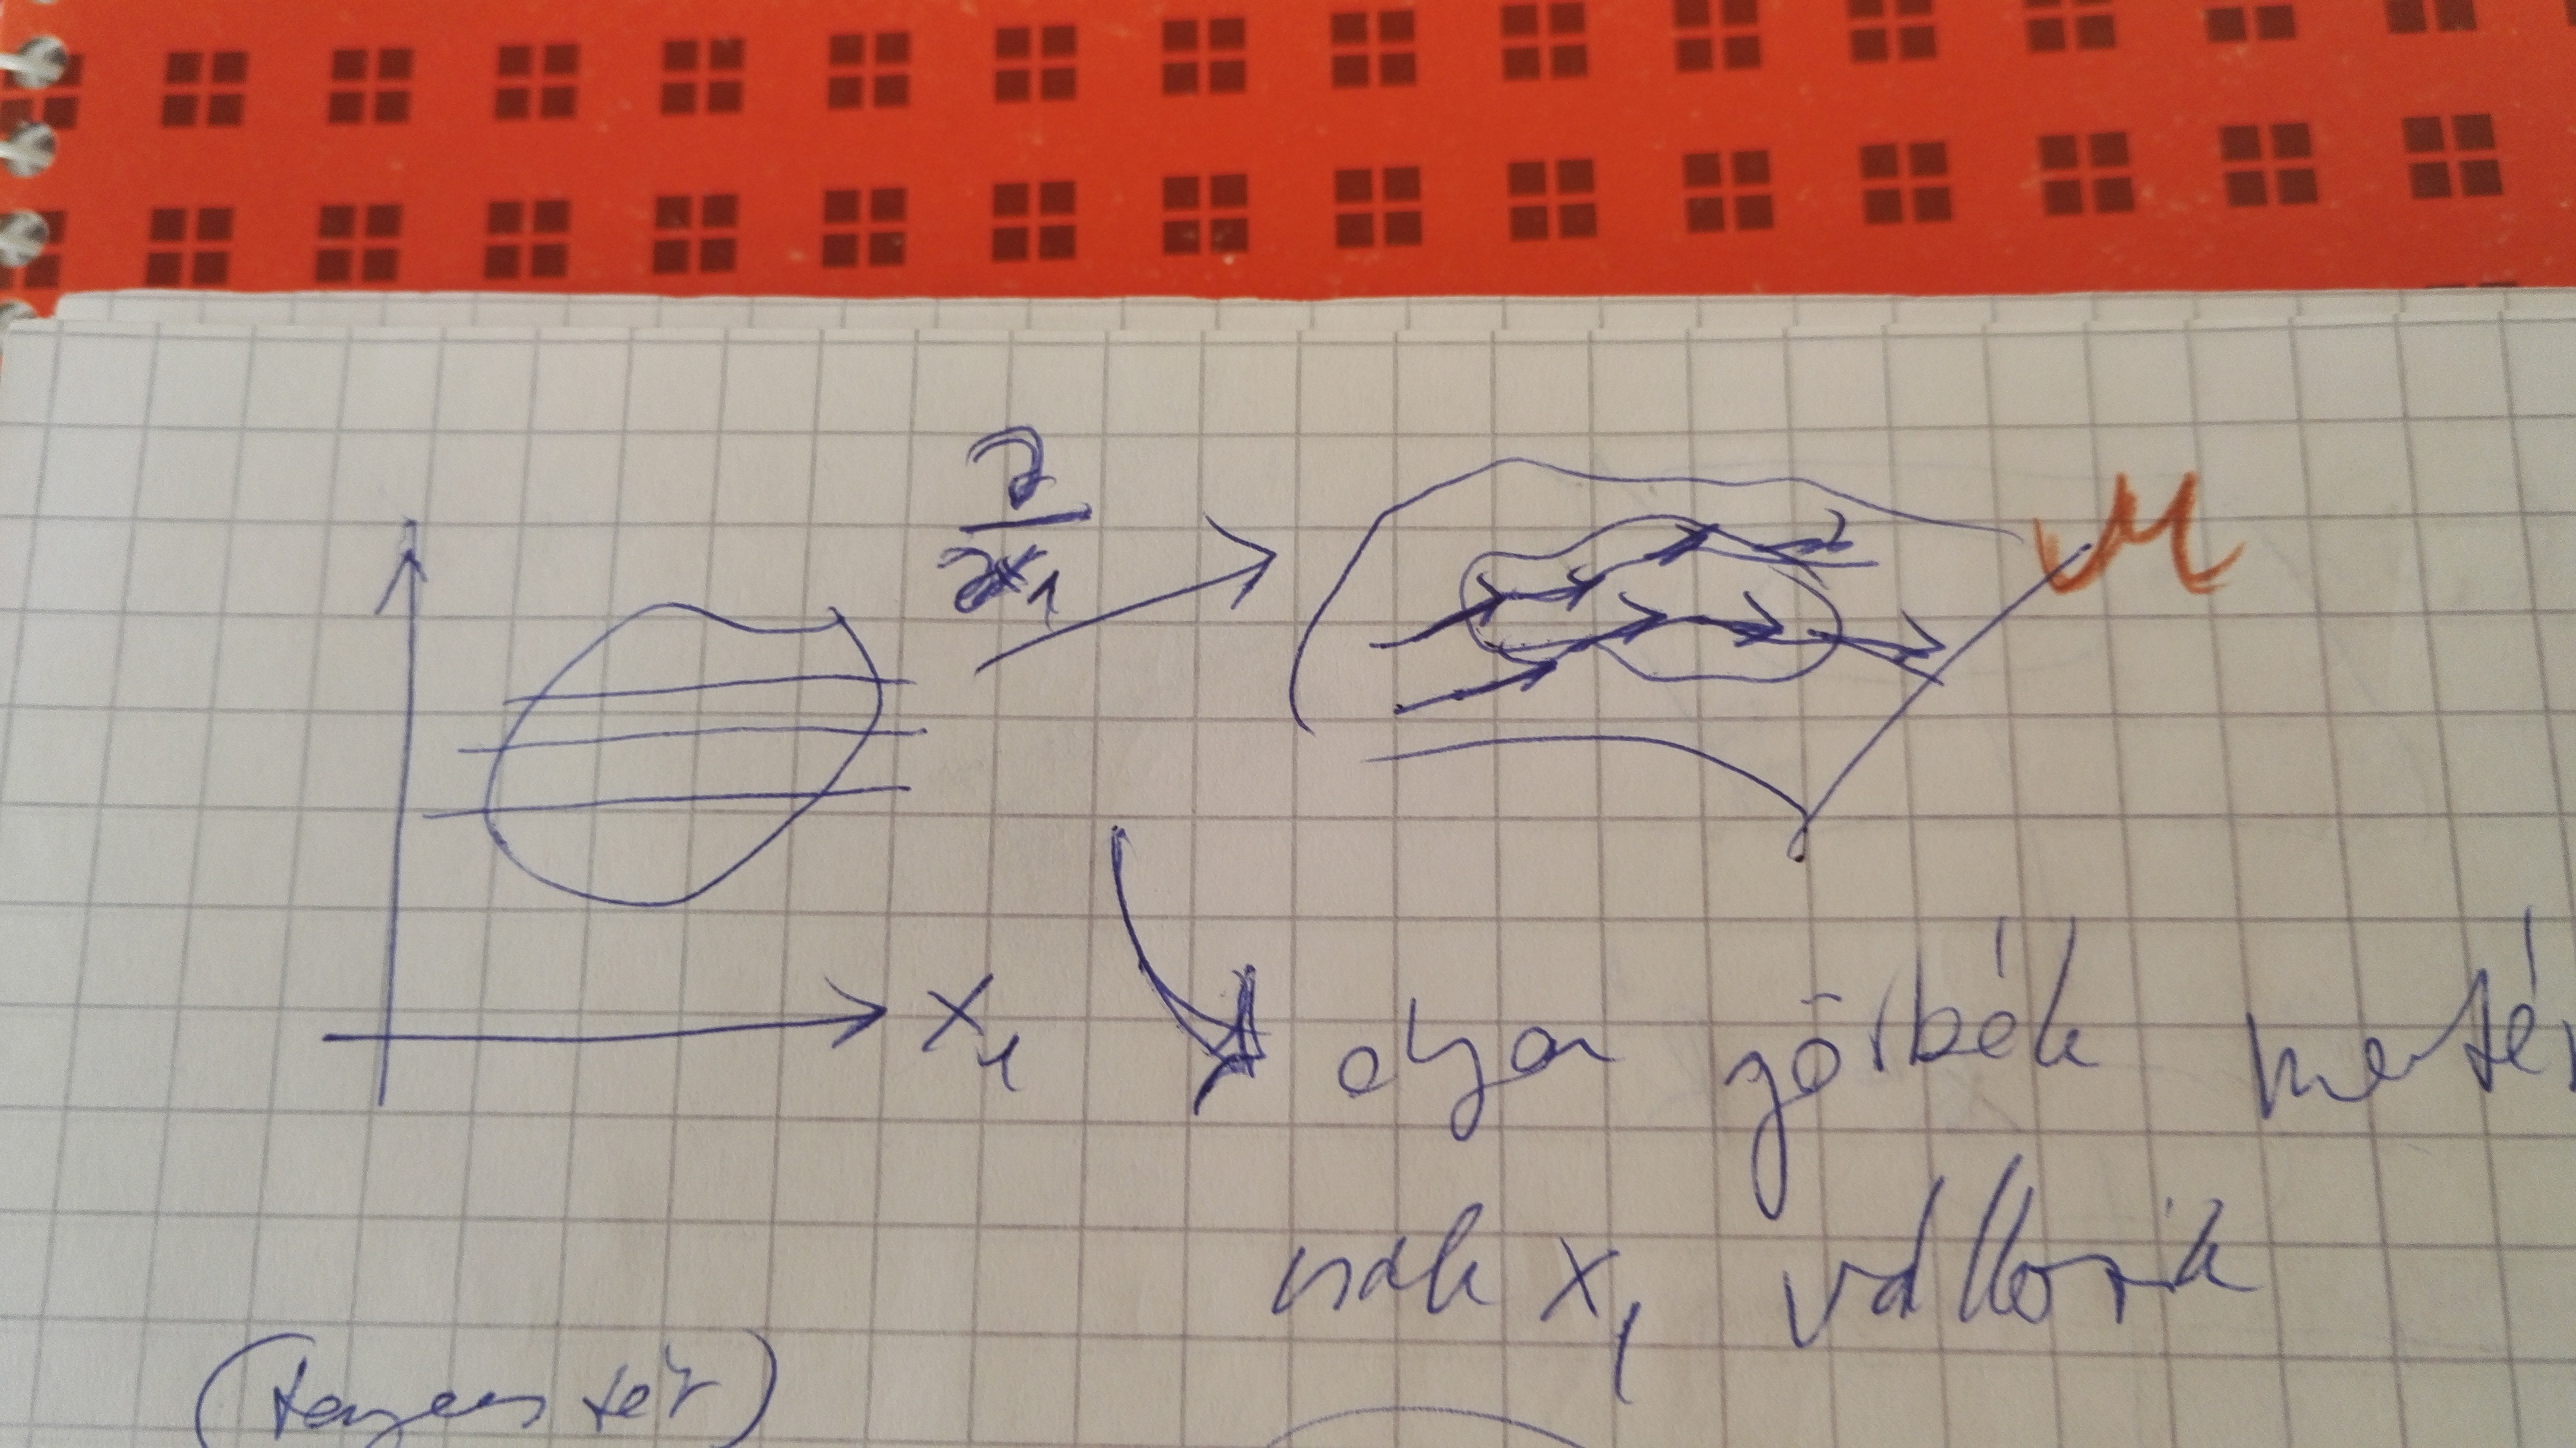
\includegraphics[width=0.9\linewidth]{derivacio.jpg}
\caption{Parciális deriváltak, mint bázisvektorok}
\end{minipage}
\end{figure}
\par Ezeket a $\partial_{k}$-kat úgy lehet szemléletesen elképzelni, hogy olyan görbék a sokaságon, amelyek paraméterezésének csak a k. koordinátája változik. Így a sokaság tangens nyalábján értelmezhető a $\textsc{kotangens nyaláb}$, amely annak duálisa. Jelöljük ezt: $T_{P}^{*}$, amely a tangens tér a sokaság $P$ pontjában, a tangens nyaláb ekkor \[U_{P\in M}^{}T^{*}_{P}\].
\par Ha készítünk kétféle paraméterezést a sokaság adott pontjában, akkor ezek között kölcsönösen egyértelmű leképezés van. A két leképezésen véve a szintvonalakat azok őse a sokaságon kijelöl görbéket. Ezen görbék mentén vett bázis vektorokkal fel lehet írni egy derivációt, mint a $\partial_{k}$-k lineáris kombinációját, hiszen ezek mind $T^{*}_{P}$-ben vannak. Tehát véve az egyik leképezésen egy skalár mezőt $\Phi(x^{k})$ és erre hattatva az előbbi derivációt a következőt:
\begin{equation*}
    D\Phi = v^{k}\frac{\partial\Phi}{\partial x^{k}}
\end{equation*}
\par Ha $\Phi(x^{k})$-t kifejezzük a másik leképezésen, akkor $\Phi(x'^{k}(x^{k}))$-n mivel kölcsönösen egyértelmű a hozzárendelés a két leképezés között, így:
\begin{equation*}
    \Psi = v^{k}\partial_{k}\Phi = v^{k}\partial_{k}(\Phi(x'(x))) = v^{k}\frac{\partial\Phi}{\partial x'^{l}}\frac{\partial x'^{l}}{\partial x^{k}}
\end{equation*}
\par Ahol a koordináták közötti két indexes mennyiséget:
\begin{equation*}
    \frac{\partial x'^{l}}{\partial x^{k}} = A^{l}_{k}(x)
\end{equation*}
\par Amivel már könnyen láthatjuk, hogy a $v^{k}$ komponensek a következőképpen transzformálódnak:
\begin{gather*}
    v'^{l} = A^{l}_{k}(x)v^{k} \\
    \Psi = v^{k}\partial_{k}\Phi = v'^{l}\partial'_{l}\Phi
\end{gather*}
\par Fontos megjegyezni, hogy $A$ egy lineáris transzformáció lokálisan, viszont globálisan hely függő, így nem tudunk globális valamilyen 'szép' leképezést adni, csak lokálisan, akkor viszont $A$ egy konstans mátrix. Ennek segítségével már kimondhatjuk, hogy vektor az ami így transzformálódik. Adott pontban már értelmezhetünk vektor mezőt. 
\par Most már tudjuk, hogy a kontra variáns (felső indexes) vektorok hogy transzformálódnak, most tehát meg kell néznünk a kovariáns (alsó indexes) trafót is.
\begin{equation*}
    u_{k}' = \frac{\partial\Phi(x(x'))}{\partial x'^{k}} = \frac{\partial\Phi}{\partial x^{l}}\frac{\partial x^{l}}{\partial x'^{k}} = B_{k}^{l}(x')u_{l}
\end{equation*}
\par $B$ szintén lokálisan lineáris trafó globálisan pedig valami 'csúnya' transzformáció, azaz nem linearizálható. Könnyen belátható, hogy $A,B$ egymás inverzei.
\begin{gather*}
    \frac{\partial x^{k}}{\partial x^{m}} = \delta^{k}_{m} \\
    \frac{\partial x^{k}}{\partial x^{m}} = \frac{\partial x^{k}}{\partial x'^{l}}\frac{\partial x'^{l}}{\partial x^{m}} = \\
    A^{k}_{l}B^{l}_{m} = \delta^{k}_{m}
\end{gather*}
\par Miután vektorok trafóját értelmeztük, értelmezhető a tenzor fogalom is. Hiszen tenzor az, ami úgy transzformálódik, mint vektor komponensek szorzata:
\begin{gather*}
    T^{kl}' = A^{k}_{p}A^{l}_{q}T^{pq} \\
    T'_{kl} = B_{k}^{p}B_{l}^{q}T_{pq} \\ \\
    T^{kl}_{m}' = A^{k}_{p} A^{l}_{q} B^{r}_{m} T^{pq}_{r}
\end{gather*}
\par Még mindig nem jutottunk el a Riemann-geometriáig, mivel nincs metrikus tenzorunk, nincsen távolság fogalmunk még. Kell egy metrikus-tenzor!
\section{Riemann-geometria, metrikus-tenzor}
\par Legyen a sokaság P pontjában $T_{P}$ lineáris érintő tér és $T^{*}_{P}$ az ehhez tartozó kotangens tér. A duális térbeli bázis szimbólumok pedig a $dx^{k}$-k lesznek. Így a potenciál megváltozása:
\begin{equation*}
    d\Phi = \partial_k \Phi dx^{k}
\end{equation*}
\par Legyen most metrikánk. Legyen $V$ vektortér és $V^{*}$ ennek duális tere. Ezekben legyenek bázisaink és egy egymásra képző műveletünk. 
\begin{align*}
    v^{k}e_{(k)} \in V \\
    u_{l}f^{(l)} \in V^{*} \\ \\
    v_{k} = g_{kl}v^{l} \quad \quad g : V \rightarrow V^{*} \\
    v^{l} = G^{lm}v_{m} \quad \quad G : V \rightarrow V^{*} \\ \\
    G = g^{-1}
\end{align*}
\par Viszont lineáris műveletet csak mezőként, itt tenzor mezőként lehet értelmezni. Tehát $g_{kl}(x)$ leképezés minden pontban értelmezett. Fizikusok között elterjedt, hogy a $g$ leképezés inverzét is $g$-vel jelölik, azaz nem különböztetik meg a terek közötti leképezéseket betűvel csak indexeikben. Legyen tehát:
\begin{equation*}
    G^{kl}(x) = g^{kl}(x) = B^{k}_{q}(x)B^{l}_{p}(x)g_{qp}(x)
\end{equation*}
\par A metrikus tenzor bevezetése teljesen önkényes. Riemann azt követelte meg, hogy $g$ legyen pozitív definit mátrix így két pont közötti távolságot mindig pozitívnak tudott definiálni. Az általános relativitás elméletben ezt elvetjük. Az pszeudo-Riemann geometriát használ, hogy megtarthassuk a térszerű, időszerű és fényszerű 'távolságokat'. Kicsiben, azaz lokálisan vissza kell kapjuk a Minkowski-teret. Ha a metrikus tenzorral definiált skalár szorzás szimmetrikus, akkor a metrikus tenzor is az.
\begin{gather*}
    u,v \in V \\
    u^{+} \in V^{*} \\ \\
    u^{+}(v) = u_{k}v^{k} = g_{kl}u^{l}v^{k}
\end{gather*}
\par Áltrelben megköveteljük, hogy a metrikus tenzor szignatúrája (3 pozitív, 1 negatív sajátérték) megmaradjon bázistrafó során. Ez kell az időszerű, térszerű és fényszerű távolságok bevezetéséhez. Ez a tulajdonság csak a koordinátázástól függ. 
\par Kis elmozgulásokra a sokaságon na pont érintő tere ahonnan az elmozdulást indítottuk közel azonosnak tekinthető a metrikus térrel. Így:
\begin{equation*}
    g_{kl}dx^{k}dx^{l} = ds^{2}
\end{equation*}
\par ívelemnégyzet definiálható. Ha $g_{kl}$ pozitív definit, akkor $\int ds$-nek mindig van értelme. Az áltrelben viszont két tetszőleges pont távolságát nem lehet értelmezni.
\par Vegyünk $R^{n}$-ben egy $w$ paraméterrel paraméterezett görbét, majd ezt 'felvetítjük' a sokaságra. Így:
\begin{gather*}
    dx^{k} = \dot{x}^{k}dw \\
    ds^{2} = g_{kl}(x(w))\dot{x}^{k}(w)\dot{x}^{l}(w)dw^{2} \\
    ds = \sqrt{g_{kl}(x(w))\dot{x}^{k}(w)\dot{x}^{l}(w)}dw \\ \\
    S = \int ds = \int_{w_{1}}^{w_{2}}f(w)dw
\end{gather*}
\par Két távoli pont távolsága csak Riemann-geometriában van értelmezve. Ennek a hatás integrálnak kell a minimumát keresni variáció számítással ($\delta S = 0$). A legutolsó képletből származtatható $Euler-Lagrange-egyenletek$el meg lehet mondani a minimális távolságot. Az általános relativitás elméletben ahhoz, hogy két távoli pont távolságát értelmezni tudjuk más módszert kell alkalmazni.
\par Vegyünk a számunkra 'most-síkokat' a térben. Lényegében megvizsgáljuk, hogy más hely lévő megfigyelőknek hogy telik az idejük, ha nekünk $dt$ idő telik el. Tegyük fel, hogy barátainkkal együtt egy helyben állunk a tér különböző pontjaiban. Ekkor az én négyes vektorom:
\begin{gather*}
   x^{k} = \Spvek{ct, x, y, z}
\end{gather*}
\par Ennek megváltozása szimplán az első koordinátám megváltozásából áll majd, mivel egy helyben állok, tehát $dx^{k} = cdt$. Az egy helyben állásnak van fizikai jelentése, így érdemes vizsgálni, hogy mi ennek a feltétele matematikailag. Ahhoz, hogy egy helyben tudjunk állni $dt$ ideig az szükséges, hogy a tér-időbeli pontjaink időszerűen legyenek elválasztva, azaz az ívelem négyzet pozitív legyen.
\begin{equation*}
    ds^{2} = g_{kl}dx^{k}dx^{l} = g_{00}dx^{0}dx^{0} + 0 = g_{00}c^{2}dt^{2}
\end{equation*}
\par Azaz kikötést kaptunk $g_{00}$ értékére, miszerint annak pozitívnak kell lennie, minden vonatkoztatási rendszerben, hogy lehessen egy helyben maradás. Ez indokolja, hogy az általános relativitás elméletben megköveteljük, hogy a metrikus tenzor szignatúra tartó legyen.
\begin{gather*}
    d\tau = \frac{1}{c}ds \\
    d\tau = \frac{1}{c}\sqrt{g_{00}c^{2}dt^{2}} \\
    d\tau = \sqrt{g_{00}(x)}dt
\end{gather*}
\par Megkaptuk tehát, hogy a sajátidő helytől függően máshogy telik az én rendszeremhez képest. A specrelben eddig ehhez arra volt szükség, hogy $Lorentz-boost$al átlépjünk egy másik rendszerbe. Itt ez a tér tulajdonsága.
\section{Metrikus tenzor a fizikában}
\par Az elmélet kiköti, hogy nem értelmezhető tenzor, csak tenzor mező. Ezek közül kitüntetünk egyet és az lesz a metrikus tenzor. Bizonyos tulajdonságokat előírunk, hogy a végén valamilyen értelmes fizikát kapjunk az egészből. Fizikus módi, hogy a metrikus tenzor inverzét ugyan azzal a betűvel jelöljük, mint magát a tenzort. 
\par Einstein elvetette a metrikus tenzor pozitív definitségét így nem értelmezhető távoli pontok távolsága. 
\par Orientálható sokaságokkal foglalkozunk. Erre pontos definíciót nem adunk. A szemléletes magyarázat az, hogy ha kiválasztunk egy jövőbe mutató vektort akkor azt nem lehet addig transzformálni, míg valamilyen rendszerben múltba tartó nem lesz. A metrikus tenzort úgy kell bevezetnünk, hogy ne legyen értelme a térszerű trajektóriának és egy világ vonal minden pontjába húzott érintő  jövőbe mutatónak kell legyen. 
\par A téridő koordinátázása önkényes, így nem kell, hogy $x_0$ koordináta időszerű legyen, sőt egyáltalán nincs szükség tisztán időszerű koordinátára. Így általában nincs konkrét jelentése kizárólag egy koordináta megváltozásának.
\par Vizsgáljuk a következő szituációt. Az űrben lebegünk két űrhajóval és megpróbáljuk szinkronizálni az óráinkat, hogy tudjuk mikor kell lecsapni az ellenségre. Ehhez mi fény jelet küldünk az űrhajóra, majd amit az megkapja vissza is küldi nekünk egyből. Miután megkapjuk az üzenetet előre állítjuk az óránkat a küldés és fogadás között, számunkra eltelt idő felével, hiszen az űrhajó állandó távolságra volt tőlünk, így az újonnan szerzett időnket tekinthetjük az űrhajó $most$jának. Most pedig számoljunk, szem előtt tartva, hogy a fény terjedése során az ívelem négyzet mindig zérus.
\begin{gather*}
    ds^{2} = g_{kl}dx^{k}dx^{l} = g_{00}dx^{0}dx^{0} + g_{0\alpha}dx^{0}dx^{\alpha} + g_{\alpha 0}dx^{0}dx^{\alpha} +
    g_{\alpha\beta}dx^{\alpha}dx^{\beta} = 0 \\
    dx^{\alpha} = konstans \\
    ds^{2} = g_{00}(dx^{0})^{2} + 2(g_{0\alpha}dx^{\alpha})dx^{0} + (g_{\alpha\beta} dx^{\alpha}dx^{\beta}) = 0
\end{gather*}
\par A másodfokú egyenlet két megoldása pontosan megadja a jel megkapásától indított fény kúp és a küldő űrhajó idő vonalának két metszés pontját, azaz a küldési és visszafogadási időpontokat. Ezek átlaga a Viete-formulákat alkalmazva:
\begin{equation}
    dx^{0}_{new} = \frac{dx_{1}^{0} + dx_2^{0}}{2} = -\frac{g_{0\alpha}}{g_{00}}dx^{\alpha}
\end{equation}
\par Viszont van egy aprócska probléma. Ez csak szomszédok között működik! Sajnos nem lehet egy egész flottát szinkronizálni. Csak akkor lehetne lehetséges, ha $g_{0\alpha} = 0$ lenne. Adott rendszerben mindig tudunk olyan metrikus tenzort konstruálni, ami ilyen, így a szinkronizálhatóság definiálható, de ez a koordinátázás tulajdonsága. Matematikailag a metrikus tenzor önkényes. Fizikailag viszont a szinkronizációból azt kapjuk, hogy valahol a múltban (Nagy Bumm) vagy a jövőben  (Nagy Reccs) szingularitást kapok. Az $Einstein-egyenletek$ből majd ez következik, de egyenlőre ez csak egy érdekes megjegyzés. 
\end{document}\grid
